\subsection*{Velocity}
I sprint 1 forventede vi at have 4 timer om dagen per mand i gruppen. Dvs. 8 mandetimer om dagen med 2 hold med
4 arbejdsdage. \\
Vi regnede os til at 5 storypoint (standard) tager 8 mandetimer \\
Det svarer til: 5 storypoints / 8 mandetimer = 0,625 storypoint per mandetime \\

32 mande timer i en iteration. \\
32 mandetimer * 0,625 = 20 storypoints per uge, dvs. 5 storypoints per dag. Dog tog vi et ekstra storypoint med for ugen.

\subsection*{Planl�gning}
Til sprintet afbillede vi vores burndown som en funktion af storypoints per mandedage. \\

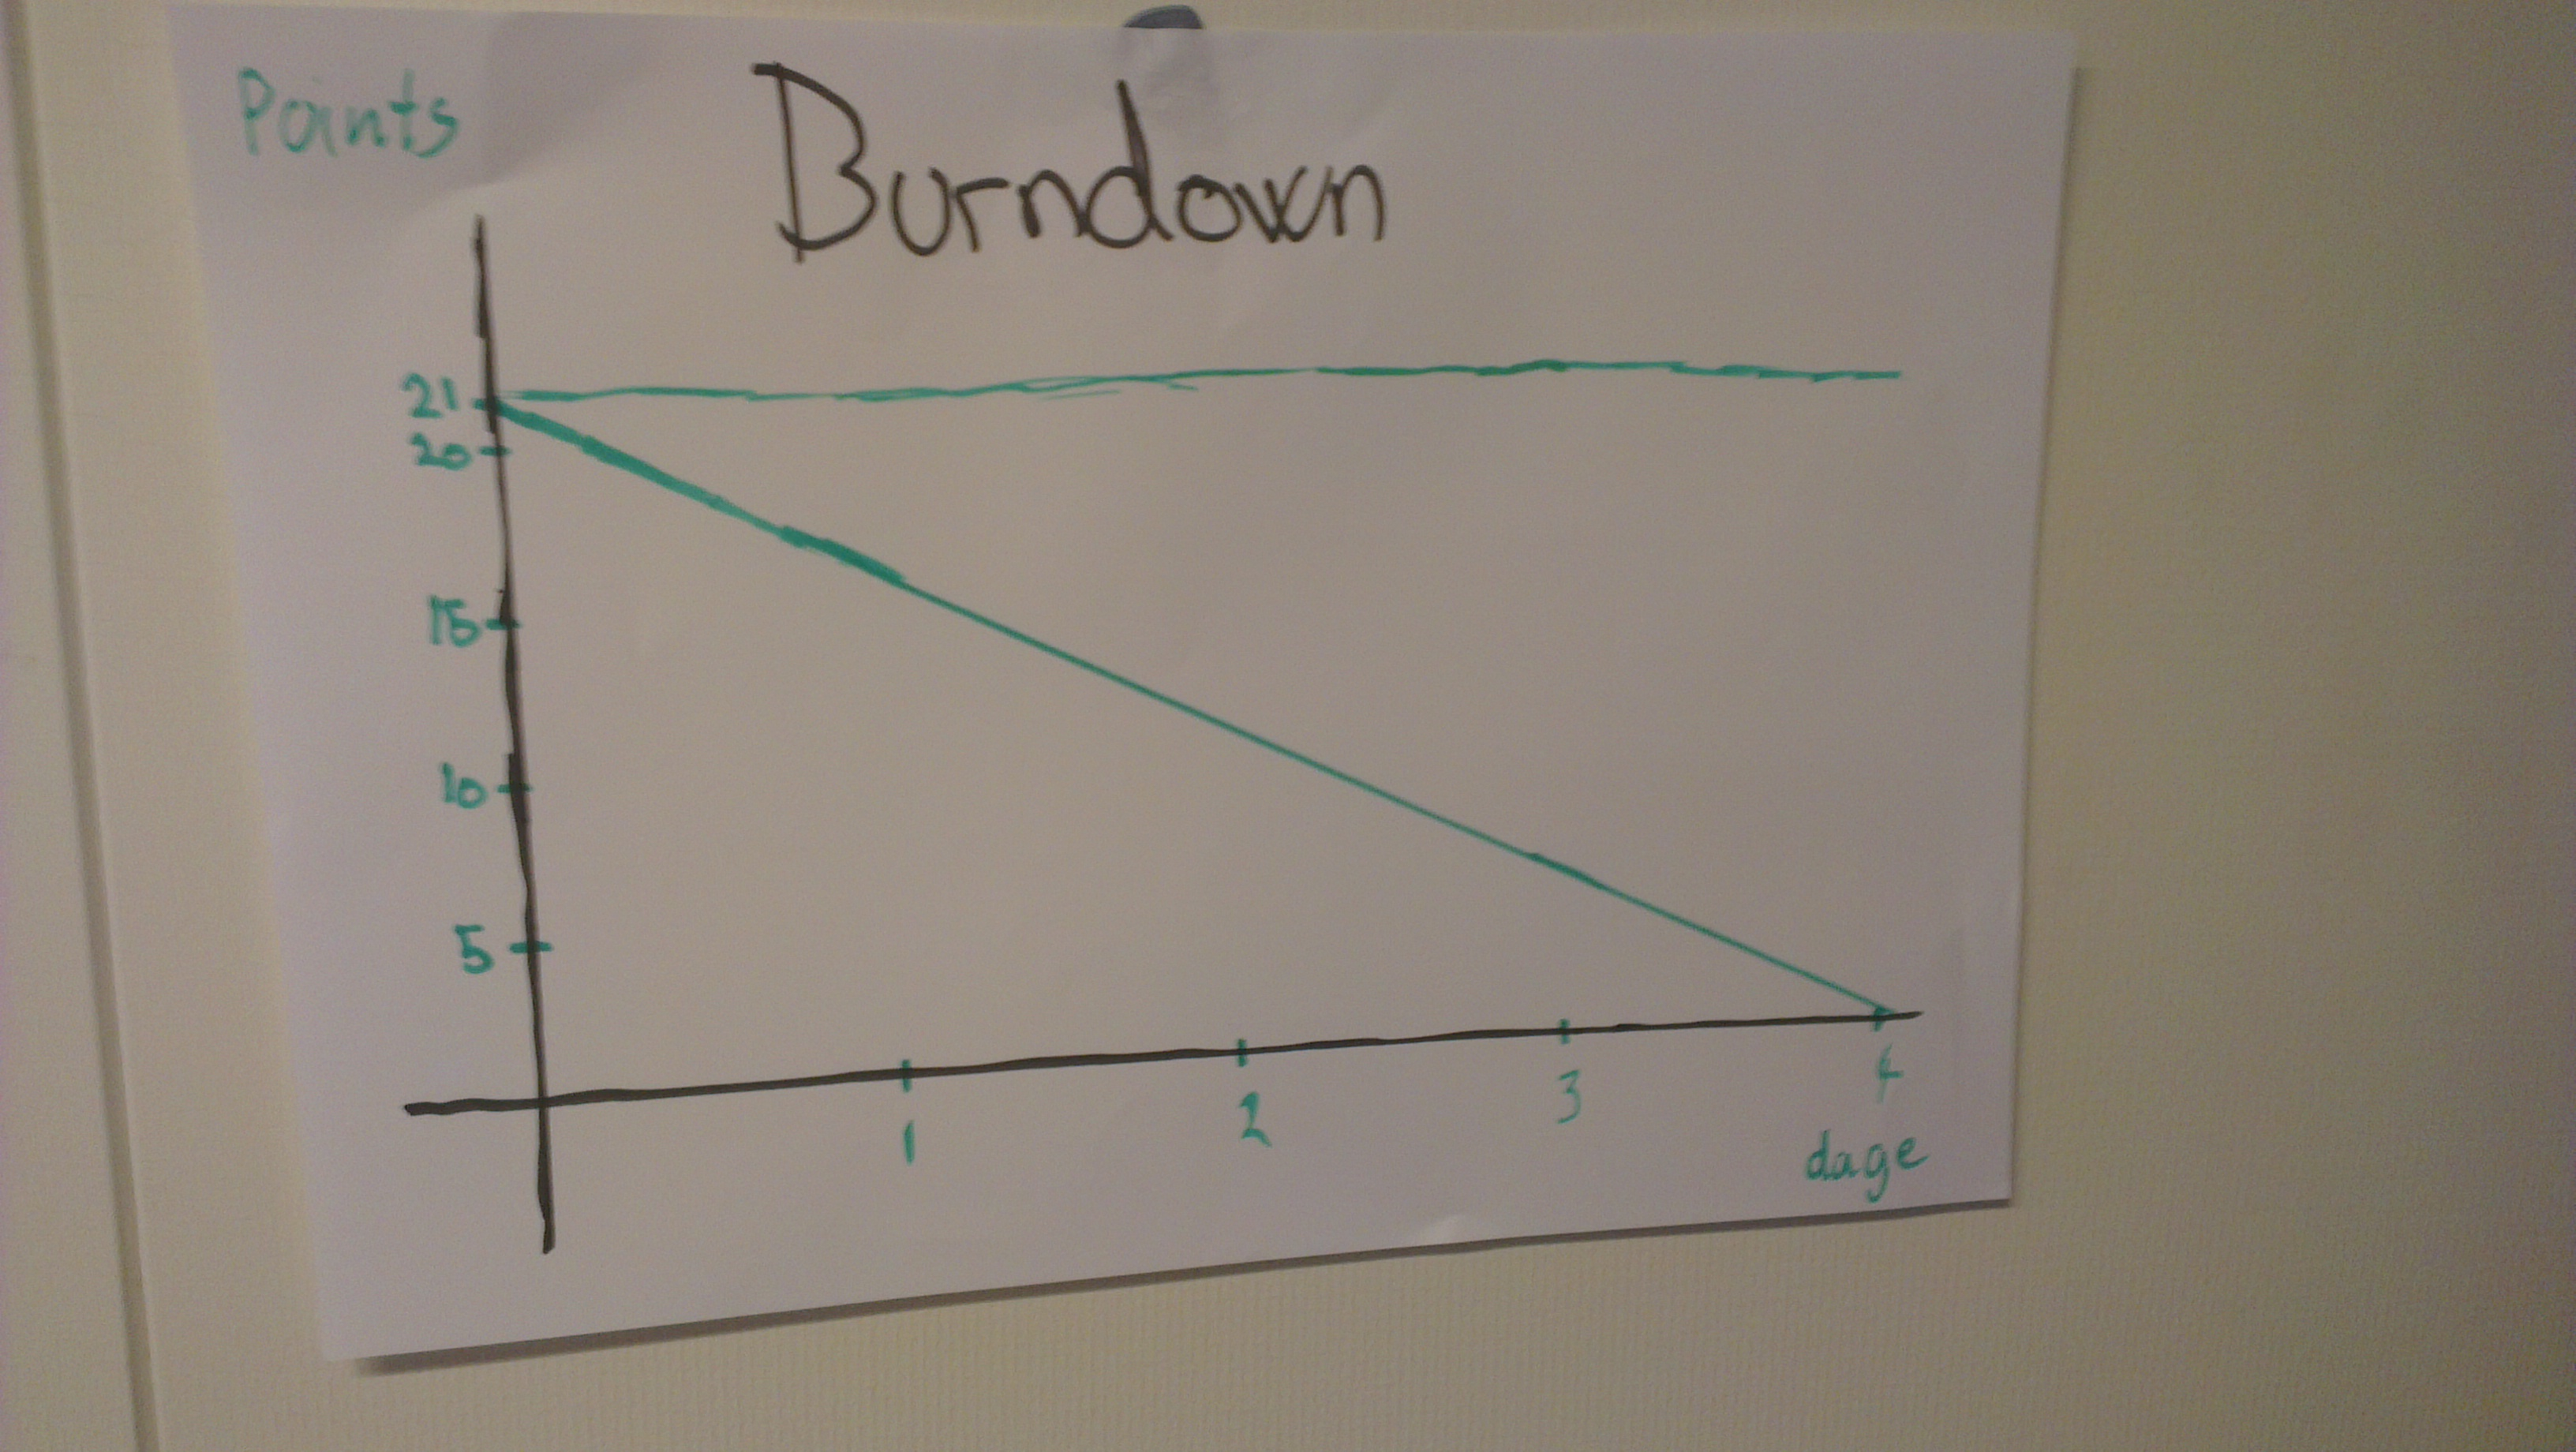
\includegraphics[scale=0.001]{includes/billeder/IMAG0021.jpg}

I sprintet fokuserede vi p� 2 userstories:
\begin{itemize}
\item Kunden vil gerne have flere forslag til ingredienser frem p� food map, ved at trykke p� den midterste knap.
\item Kunden vil gerne have adgang til database.
\end{itemize}

I disse userstories omhandlede tasks med: 
\begin{itemize}
\item database design
\item oprettelse af tabeller
\item gui samt generel funktionalitet til foodmap
\end{itemize}


Backloggen s� i sprint 1 s�dan ud:
%link til at genere tabeller: http://www.tablesgenerator.com/
\begin{table}[h]
\begin{tabular}{llll}
Userstory                                                                                                                                                                    & \begin{tabular}[c]{@{}c@{}}Story-\\ points\end{tabular} & \begin{tabular}[c]{@{}c@{}}Mande-\\ timer\end{tabular} & Prioritet                \\ \hline
\multicolumn{1}{|l}{\begin{tabular}[c]{@{}c@{}}Kunden vil gerne have flere forslag til\\ ingredienser frem p� food map, ved at\\ trykke p� den midterste knap.\end{tabular}} & \multicolumn{1}{|l}{3}                                  & \multicolumn{1}{|l}{3}                                 & \multicolumn{1}{|l|}{1}  \\ \hline
\multicolumn{1}{|l}{\begin{tabular}[c]{@{}c@{}}Kunden vil have et animeret foodmap, \\ hvor ingredienser popper ud fra den\\ eksisterende ingrediensbobbel.\end{tabular}}    & \multicolumn{1}{|l}{}                                   & \multicolumn{1}{|l}{}                                  & \multicolumn{1}{|l|}{2}  \\ \hline
\multicolumn{1}{|l}{\begin{tabular}[c]{@{}c@{}}Kunden vil gerne kunne fjerne og tilf�je\\ ingredienser i food map.\end{tabular}}                                             & \multicolumn{1}{|l}{}                                   & \multicolumn{1}{|l}{}                                  & \multicolumn{1}{|l|}{3}  \\ \hline
\multicolumn{1}{|l}{\begin{tabular}[c]{@{}c@{}}Kunden vil gerne have en liste over forskellige\\ opskrifter som er udvalgt af \\ de anf�rte ingredienser.\end{tabular}}      & \multicolumn{1}{|l}{}                                   & \multicolumn{1}{|l}{}                                  & \multicolumn{1}{|l|}{4}  \\ \hline
\multicolumn{1}{|l}{\begin{tabular}[c]{@{}c@{}}Kunden vil gerne have hurtig s�geforslag \\ til ingredienser. (Performance)\end{tabular}}                                     & \multicolumn{1}{|l}{}                                   & \multicolumn{1}{|l}{}                                  & \multicolumn{1}{|l|}{5}  \\ \hline
\multicolumn{1}{|l}{\begin{tabular}[c]{@{}c@{}}Kunden vil gerne have listet opskrifter med\\ billeder, beskrivelse, ingredienser og \\ tilberedning.\end{tabular}}           & \multicolumn{1}{|l}{}                                   & \multicolumn{1}{|l}{}                                  & \multicolumn{1}{|l|}{6}  \\ \hline
\multicolumn{1}{|l}{\begin{tabular}[c]{@{}c@{}}Kunden vil gerne kunne f� et hurtigt overblik\\  over indk�bs- og pr�perationsliste ved opskrift.\end{tabular}}               & \multicolumn{1}{|l}{}                                   & \multicolumn{1}{|l}{}                                  & \multicolumn{1}{|l|}{7}  \\ \hline
\multicolumn{1}{|l}{\begin{tabular}[c]{@{}c@{}}Kunden vil gerne have en menu til navigering\\ i appen.\end{tabular}}                                                         & \multicolumn{1}{|l}{}                                   & \multicolumn{1}{|l}{}                                  & \multicolumn{1}{|l|}{8}  \\ \hline
\multicolumn{1}{|l}{\begin{tabular}[c]{@{}c@{}}Kunden vil gerne kunne gemme indk�bsliste\\ i indk�bsoversigt.\end{tabular}}                                                  & \multicolumn{1}{|l}{}                                   & \multicolumn{1}{|l}{}                                  & \multicolumn{1}{|l|}{9}  \\ \hline
\multicolumn{1}{|l}{\begin{tabular}[c]{@{}c@{}}Kunden vil gerne kunne gemme opskrifter i\\ favoritter.\end{tabular}}                                                         & \multicolumn{1}{|l}{}                                   & \multicolumn{1}{|l}{}                                  & \multicolumn{1}{|l|}{10} \\ \hline
\multicolumn{1}{|l}{\begin{tabular}[c]{@{}c@{}}Kunden vil gerne have en s�rskilt indk�bsliste,\\  som kan tilg�s fra hovedmenuen.\end{tabular}}                              & \multicolumn{1}{|l}{}                                   & \multicolumn{1}{|l}{}                                  & \multicolumn{1}{|l|}{11} \\ \hline
\end{tabular}
\end{table}

\subsection*{Xp praktikker}
I sprint 1 benyttede vi XP praktikkerne: planning poker, par programmering, kollektivt kode ejerskab, refactoring, kodestandarder, metafor og simpelt design. \\

Vi lavede planning poker med storypoints til at vurdere st�rrelsen af userstories for senere hen at udregne vores velocity. \\
Vi arbejdede med par programmering i 2 grupper, hvor vi ogs� i h�j grad havde den af grupperne med en mand i til at unders�ge teknologien. Vi fors�gte s� vidt muligt at f� alle ind over koden hvor vi i forvejen havde aftalt at bruge Java camelcasing samt at refactorer koden med KISS som m�l.
Derudover vi benyttede dom�ne model og database schema til design for at f� enighed om samt overblik over dom�net. 

Mht. kvalitetssikring valgte vi ikke at benytte test-first eller unit testing eftersom vi p� dette tidspunkt ikke rigtigt havde noget relevant at teste p� samt at vi prioriterede funktionalitet.


\subsection{Produkt review}
Til reviewet i starten af sprint 2 pr�senterede vi vores grafiske brugergr�nseflade: 
% inds�t screenshot her.
 
\subsubsection*{Konklusion af review}
At vi havde et lovende interface med statisk funktionalitet, men uden database adgang.


\subsection*{Retrospektive}
Vi l�b ind i et problem med at vores userstory for databasen, hvilken var for bredt defineret. Dette resulterede i at vi ikke kunne tegne vores burndown ned overhovedet. 

\subsubsection*{Ting der gik godt}
Par programmering \\
Kollektivt kode ejerskab.



\subsubsection*{Mindre godt}
Vores opsplitning af user stories: \\
Vores user stories skal splittes mere og bedre op, s� vi er istand til at tegne burndown ned.
Burndown som er sammensat ved point og dage.
skriv logbog hver dag.
Korrigere for frav�r.


Andet
Vi lavede ikke test-first - Dette var ikke muligt da vi ikke er erfarne med android

Ting vi forts�tter med
Vi forts�tter med pair-progamming til de mere komplekse tasks

Ting vi vil forbedre
Burndown sammensat af timer og dage, i stedet for point.
Opdeling af user stories
Vil lave burndown af tasks istedet for user stories
Vores accept tests.